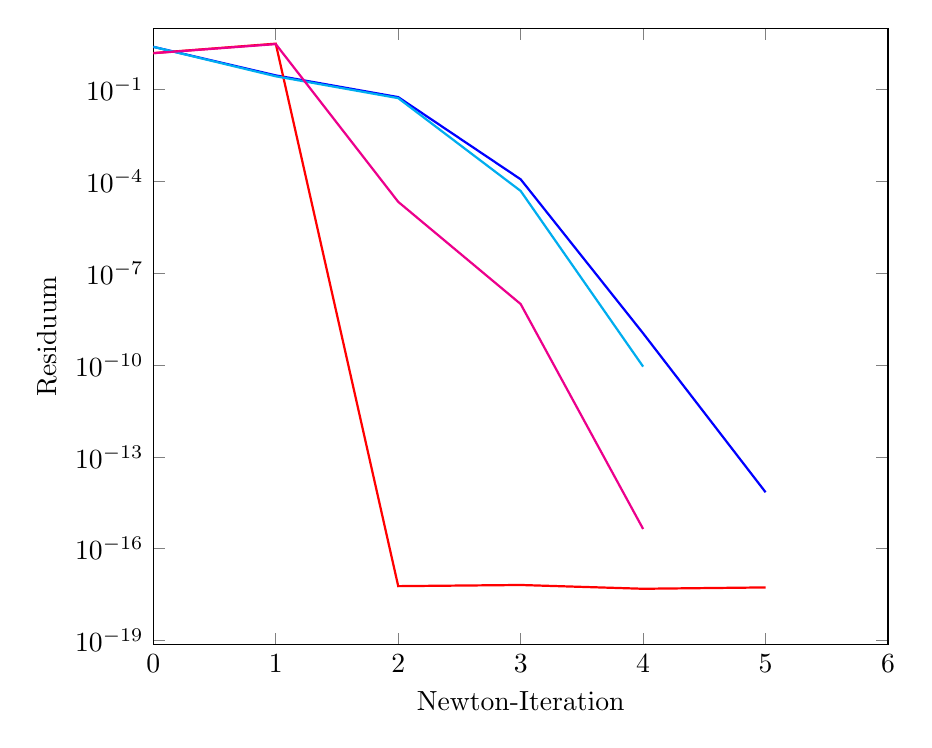
\begin{tikzpicture}[every plot/.append style={thick}] 
\begin{axis}[ 
label style={font=\normalsize}, 
xlabel={Newton-Iteration}, 
ylabel={Residuum}, 
xmin=0, xmax=6, 
ymode=log, 
ymin=0, ymax=10, 
width=0.9\textwidth, 
grid style=dashed, 
] 
\addplot[ 
color=blue, 
] 
coordinates { 
(0, 2.47e+00)(1, 2.88e-01)(2, 5.62e-02)(3, 1.16e-04)(4, 1.08e-09)(5, 6.95e-15)}; 
\addplot[ 
color=red, 
] 
coordinates { 
(0, 1.54e+00)(1, 3.13e+00)(2, 5.96e-18)(3, 6.50e-18)(4, 4.89e-18)(5, 5.41e-18)}; 
\addplot[ 
color=cyan, 
] 
coordinates { 
(0, 2.47e+00)(1, 2.69e-01)(2, 5.20e-02)(3, 4.83e-05)(4, 8.83e-11)}; 
\addplot[ 
color=magenta, 
] 
coordinates { 
(0, 1.53e+00)(1, 3.03e+00)(2, 2.13e-05)(3, 9.77e-09)(4, 4.39e-16)}; 
\end{axis} 
\end{tikzpicture} 
